%model-specify.v1

The state-space model (\cf.~\Fig{fig:model}) requires as input:
\begin{enumerate}
  \item The fMRI data (projected into the low-dimensional
  feature-space), described in \Chap{chap:feature-space}.
  \item Information about the stimulus presentation timing,
  described next.
\end{enumerate}

\begin{figure}
\centering
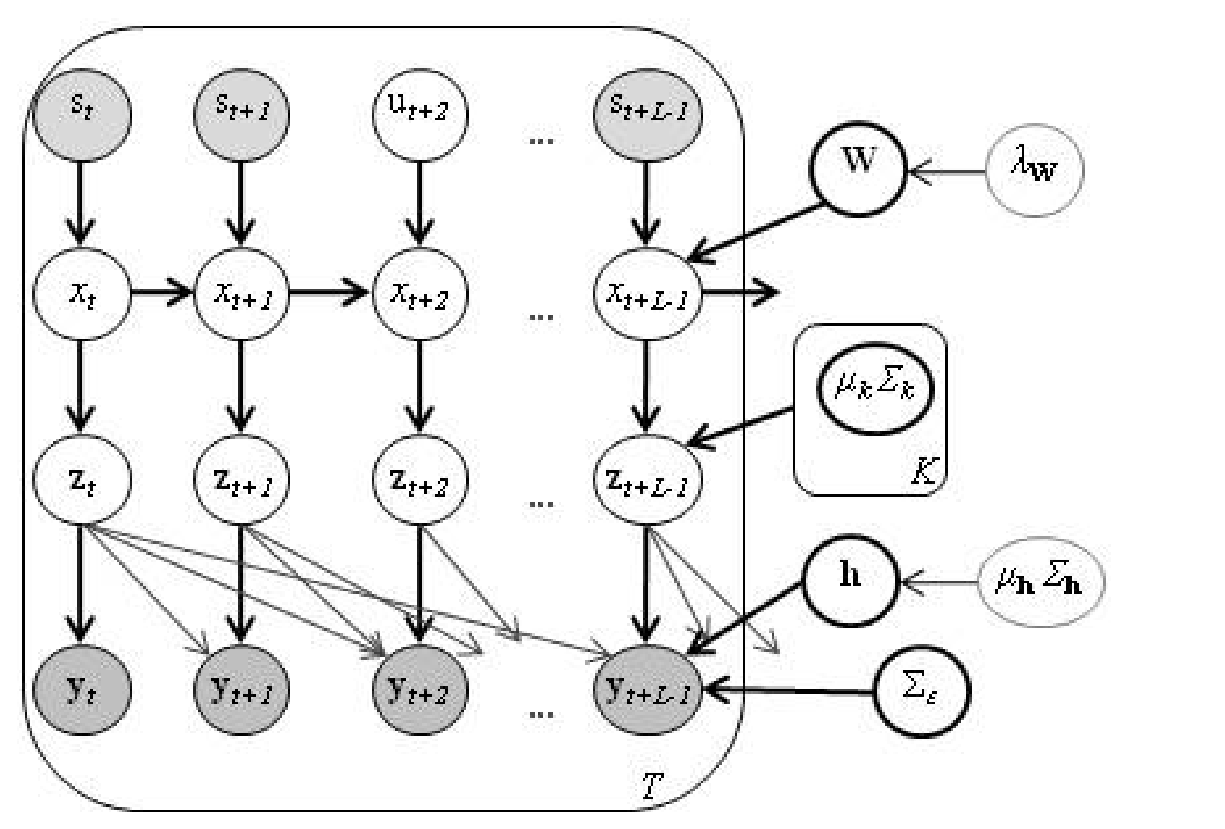
\includegraphics[width=.75\linewidth]{model}
    \caption[The State--Space Model (SSM)]{\textbf{The State--Space Model (SSM).
    } The experimental parameters are represented by $\s_t$,
    while the corresponding brain--state is $\X_t$, and
    the instantaneous activation pattern is $\Z_t$.
    The activation pattern is observed in the fMRI data $\Y_t\ldots
    \Y_{t+L-1}$  after convolution with the HRF $\h$.
    \label{fig:model}
    }
\end{figure}


A certain amount of information about the experimental paradigm can
be provided as input to the SSM estimation routines, in order to
stabilize estimation and provide a reference for estimating the
model hyper-parameters (using prediction error, measured through
cross-validation). In general, if an experiment has multiple types
(channels) of stimuli and subject responses prevalent during its
course, only some of these channels may be included in the model
estimation, as necessary. The effect of the remaining experimental
parameters on the SSM can be tested post-hoc, i.e.~after the model
has been estimated. The reader is referred to
\cite{Janoos2010g,Janoos2011} for more details on this.

\section{Specifying the Experimental Design}
\label{sec:specify}
The experimental design, to be provided as input to the
model-specification, is specified using the \verb"Specify 1-st Level"
feature of SPM (\cf.~\Fig ). Please refer to the SPM
Manual~\cite{TheFILMethodsGroup2011} for more details.

Of interest are the different conditions, their presentation timing
and duration. The rest of the fields may be filled with filler or
dummy values. Save the \verb"Specify 1-st Level" batch job as a
\verb".mat" file. This \verb".mat" is provided as input the SSM
estimation routine. There is no need to run the job - as the
\verb"SPM.mat" containing the design matrix \emph{is not used}.

\begin{figure}
\centering
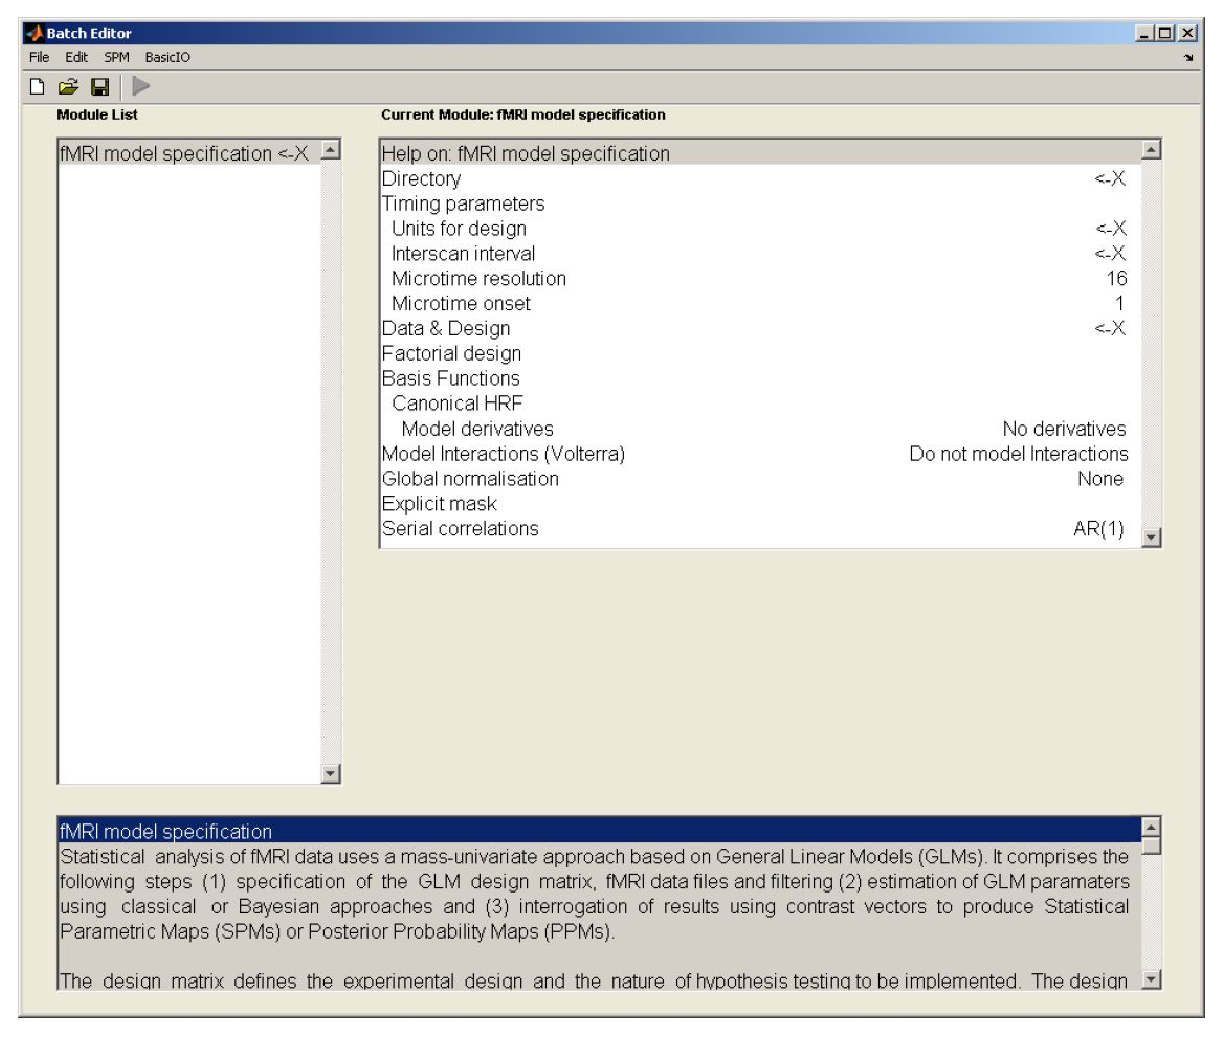
\includegraphics[width=.75\linewidth]{spm-specify}
    \caption[Specifying the Experimental Design.]
    {\textbf{Specifying the Experimental Design.}
    Use the ``Specify 1-st Level'' of SPM to specify the
    experimental conditions and the timing.
    \label{fig:specify}
    }
\end{figure}

%%  \item The length of a block of missing stimuli (in TR units)
%%  for the cross validation method of hyper-parameter selection
%%  \item The number of cross-validation iterations


\section{Estimating the Model}

To estimate the model, and do hyper-parameter selection, the following function
is used:

Function Syntax:
\begin{verbatim}
    [error_missing, log_likelihood, params_opt ]
        = ssmEstimateFull(fs_coords, specify_mat_file,
                          num_cvs, block_length,
                          tol);
\end{verbatim}
Arguments:
\begin{itemize}
  \item \verb"fs_coords" - The feature-space embedding of the fMRI session
  \item \verb"specify_mat_file" - The name of the \verb"Specify 1-st spm Level"
   job batch file (\verb".mat" format) created in \Sec{sec:specify}.
  \item \verb"num_cvs" - (Optional, Default 5) Number of cross validation steps for hyper-parameter selection.
  Typically set between 5--10.
  \item \verb"block_length" - (Optional, Default 5)  The length of a block of missing stimuli (in TR units)
     for the cross validation method of hyper-parameter selection. Typically set
     between 4 -- 8.
  \item \verb"tol" - (Optional) The relative tolerance of the various
  parameter updates specifying the termination criteria for iterative optimization. Typically
  set at 0.001 (indicating termination for a 0.1\% change in parameter value).
\end{itemize}`
Returns:
\begin{itemize}
    \item \verb"error_missing" - An array giving the distribution of the missing stimulus prediction
    error rate (over multiple cross validations) for the optimal model.
    \item \verb"log_likelihood" - An array giving the distribution of the data log
    likelihood (over multiple cross validations) for the optimal model.
    \item \verb"params_opt" - A structure of the SSM parameters averaged multiple CVs for the optimal model.
    It contains the fields:
    \begin{itemize}
      \item \verb"K_opt" - Optimal model size (number of states).
      \item \verb"lambda_opt" - Optimal value of the hyper-parameter controlling the
      estimation of the state-transition    parameters.
      \item \verb"lambda_opt" - Optimal value of the hyper-parameter controlling the
      estimation of the state-transition    parameters.
      \item \verb"w" - The 3-d array giving the state transition parameters $\mathbf{w}$,
      where \verb"w(i,j,:)" = $\mathbf{w}_{i,j}$.
      \item \verb"omega" - The 2-d array giving the state transition parameters $\omega$,
      where \verb"omega(i,:)" = $\omega_{i}$.
      \item \verb"mu" - An 2-d matrix where each column gives the mean value of the activation
      patterns corresponding to each state.
      \item \verb"Sigma" - An 3-d matrix where each 2-d sub-matrix gives the variance for each state.
      \item \verb"h" - An 2-d matrix where each column gives the estimated hemodynamic response filter
      for each element of the feature (data embedding) space.
      \item \verb"Sigma_eps" - A 2-d matrix giving the noise variance in the activation patterns.
    \end{itemize}
\end{itemize}

It is also possible to estimate the model for a given setting of the
hyper-parameters, and a given subset of the stimulus marked as hidden (unobserved) using the function described
next:
Function Syntax:
\begin{verbatim}
    [error_missing, log_likelihood, params ]
        = ssmEstimate(fs_coords, specify_mat_file,
                          t_missing, K, lambda,  tol);
\end{verbatim}
Arguments:
\begin{itemize}
  \item \verb"t_missing" - A vector of binary values the length of the session with $1$ indicating which time-point to treat
  as missing / hidden stimulus.
\end{itemize}`
